\documentclass[11pt,letterpaper]{article}
\usepackage[T1]{fontenc}
\usepackage{lmodern,amsmath,amssymb,amsthm,booktabs,microtype}
\usepackage[margin=.9in,top=.82in,bottom=.85in]{geometry}
\usepackage{xcolor,tikz}
\usepackage[colorlinks=true,allcolors=teal!65!black,
 pdftitle={Gram determinants of honeycomb hexagons and Aztec rectangles},
 pdfauthor={Blake Stone}]{hyperref}
\definecolor{ink}{HTML}{153D44}
\definecolor{accent}{HTML}{00796F}
\definecolor{rust}{HTML}{984821}
\newtheorem{theorem}{Theorem}[section]
\newtheorem{lemma}[theorem]{Lemma}
\newtheorem{corollary}[theorem]{Corollary}
\newcommand{\ii}{\mathrm i}
\newcommand{\Z}{\mathbb Z}
\newcommand{\C}{\mathbb C}
\newcommand{\N}{\mathbb Z_{\ge0}}
\newcommand{\Gram}{\mathcal D}
\newcommand{\Mac}{\mathop{\rm Mac}}
\newcommand{\coeff}[1]{[#1]}
\newcommand{\minorblock}{\mathcal B}
\newcommand{\tr}{\operatorname{tr}}
\setlength{\parindent}{1.15em}
\raggedbottom
\begin{document}
\begin{center}
{\Large\bfseries\color{ink} Gram determinants of honeycomb hexagons\\[2pt] and Aztec rectangles}\\[7pt]
{\large Propp's Problems 26 and 27 and the eigenvalue \(4\)}\\[8pt]
Blake Stone\\[-1pt]{\small Proof developed with OpenAI Codex}
\end{center}
\begin{abstract}
We evaluate the Kasteleyn--Percus Gram determinant for every honeycomb hexagon, Aztec rectangle and fool's rectangle. For a hexagon the answer uses a Gram matrix whose order is the color imbalance. For an Aztec rectangle it is a product of two Toeplitz minors with an explicit finite root formula. For a fool's rectangle we obtain the entire spectrum. The eight historical fool's-diamond entries are the positive square roots of the determinants, and the two parity products conjectured by Seiichi Manyama follow. We also determine the exact multiplicity of the eigenvalue \(4\) on every Aztec rectangle, explaining an observation of Nicolau Saldanha.
\end{abstract}

\section{The graphs and the determinant}
For a finite planar bipartite graph, take a Kasteleyn--Percus matrix \(K\) with the smaller color class indexing its rows and entries of modulus one on edges. Write
\(\Gram=\det(KK^*)\), where \(K^*\) is conjugate transpose. Empty determinants and empty products equal one. In the balanced case \(\Gram\) is the square of the number of perfect matchings. The rectangular matrix still has a Gram determinant when the two colors have different sizes. Changing phases at vertices conjugates \(KK^*\) by a diagonal unitary matrix, so preserves \(\Gram\).

Problems 26 and 27 in Propp's 1999 list ask for this determinant in three families \cite[pp.~282--283]{propp}. Propp gives a honeycomb example, records Matt Blum's Aztec-rectangle formulas for short sides \(1,2,3\), and tabulates eight fool's-diamond values. We keep the indexing of the pictured order-three fool's diamond. Related results include Knuth's checkerboard spanning-tree formulas \cite{knuth}, Saldanha's singular polynomials \cite{saldanha}, and Manyama's parity conjectures in A071102 \cite{oeis}. The results below give explicit evaluations for all positive side lengths.

\begin{center}
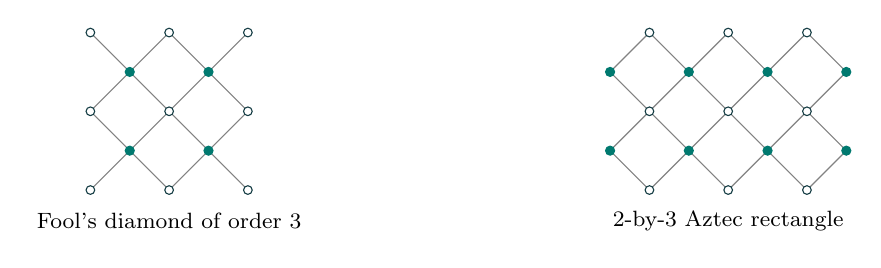
\begin{tikzpicture}[x=.50cm,y=.50cm,baseline=(current bounding box.center)]
\begin{scope}
\foreach \u in {1,3} \foreach \v in {1,3} {
  \foreach \du in {-1,1} \foreach \dv in {-1,1} {
    \draw[black!49] (\u,\v)--({\u+\du},{\v+\dv});}
}
\foreach \u in {0,2,4} \foreach \v in {0,2,4} \filldraw[fill=white,draw=ink] (\u,\v) circle (.11);
\foreach \u in {1,3} \foreach \v in {1,3} \fill[accent] (\u,\v) circle (.13);
\node at (2,-.78) {\footnotesize Fool's diamond of order \(3\)};
\end{scope}
\begin{scope}[xshift=6.6cm]
\foreach \u in {1,3} \foreach \v in {0,2,4,6} {
  \foreach \du in {-1,1} \foreach \dv in {-1,1} {
    \pgfmathtruncatemacro{\w}{\v+\dv}
    \ifnum\w>0 \ifnum\w<6 \draw[black!49] (\v,\u)--(\w,{\u+\du});\fi\fi}
}
\foreach \u in {0,2,4} \foreach \v in {1,3,5} \filldraw[fill=white,draw=ink] (\v,\u) circle (.11);
\foreach \u in {1,3} \foreach \v in {0,2,4,6} \fill[accent] (\v,\u) circle (.13);
\node at (3,-.78) {\footnotesize \(2\)-by-\(3\) Aztec rectangle};
\end{scope}
\end{tikzpicture}
\end{center}
\noindent In these rotated square-lattice coordinates the filled vertices index the rows. An edge whose two coordinate changes have the same sign receives weight \(1\). The other edges receive \(\ii=\sqrt{-1}\). Around every elementary square the two alternating products have ratio \(-1\), as required.

\clearpage
\section{Fool's rectangles and the missing square}
A fool's rectangle \(F_{r,s}\) has \(rs\) cell centers and the \((r+1)(s+1)\) grid corners incident to them. Each center sees its four corners. Propp's order \(n\) is \(F_{n-1,n-1}\). Let \(P_r\) be the adjacency matrix of the path on \(r\) vertices.
\begin{theorem}\label{th:fool}
For \(r,s\ge0\), the Gram matrix of \(F_{r,s}\) is \(4I+P_r\otimes P_s\) in cell coordinates. In particular
\[
 \Gram(F_{r,s})=\prod_{j=1}^{r}\prod_{k=1}^{s}
 \left(4+4\cos\frac{\pi j}{r+1}\cos\frac{\pi k}{s+1}\right).
\]
The factors give the full spectrum with multiplicities.
\end{theorem}
\begin{proof}
Each row has squared length four. Cells sharing a side share two corners, whose contributions to the row inner product are \(\ii\) and \(-\ii\). Diagonally adjacent cells share one corner with inner product \(1\). All other pairs have disjoint supports. This gives the matrix identity. The vectors with coordinates \(\sin(\pi j\ell/(r+1))\), \(1\le\ell\le r\), have path eigenvalues \(2\cos(\pi j/(r+1))\) by the sine addition formulas and the two zero endpoint values. They form a basis because they are nonzero and have distinct eigenvalues. Tensor products give the displayed list.
\end{proof}
Put \(u=\lfloor r/2\rfloor,\ v=\lfloor s/2\rfloor,\ z=rs-4uv\). Define the monic integer polynomial
\[
 Q_r(x)=\sum_{j=0}^{u}(-1)^j\binom{r-j}{j}x^{u-j}.
\]
The path characteristic polynomial is \(x^{r\bmod2}Q_r(x^2)\) by the continuant recurrence \(p_r=xp_{r-1}-p_{r-2}\), \(p_0=1,\ p_1=x\). Its nonzero roots are the pairs \(\pm\sqrt{\alpha}\) for \(Q_r(\alpha)=0\). The four sign choices for each \((\alpha,\beta)\) contribute \((16-\alpha\beta)^2\). The remaining \(z\) factors are four. Thus
\begin{equation}\label{eq:resultant}
 R_{r,s}:=\sqrt{\Gram(F_{r,s})}
 =2^z\!\!\prod_{Q_r(\alpha)=Q_s(\beta)=0}(16-\alpha\beta)\quad\in\Z_{>0}.
\end{equation}
The product runs over all pairs of roots and is an integer by symmetry in the roots of each monic integer polynomial. Positivity follows from \(0<\alpha,\beta<4\).
\begin{corollary}[Manyama's two parity products]\label{th:manyama}
Write \(a(n)=R_{n-1,n-1}\) and \(L(h,t)=\prod_{1\le j,k\le h}
(1-\cos^2(\pi j/t)\cos^2(\pi k/t))\). Then
\[
 a(2h+1)=4^{2h^2}L(h,2h+1),\qquad
 a(2h)=2\,4^{2h(h-1)}L(h-1,2h).
\]
\end{corollary}
\begin{proof}
In \eqref{eq:resultant}, \(\alpha_j=4\cos^2(\pi j/n)\). For odd \(n\) one has \(z=0\). For \(n=2h\) one has \(z=4h-3\). Extracting \(16\) from each factor gives both prefactors.
\end{proof}
These are the products conjectured for the tabulated sequence in A071102 \cite{oeis}. The literal determinant at order two is \(4\), since \(K\) is a single row of four unit entries. At order three the spectrum is \(3,3,5,5\) and the determinant is \(225\). Propp's corresponding entries \(2\) and \(15\) specify the normalization.

\clearpage
\section{Honeycomb hexagons}
We use a determinant identity that also controls the Aztec rectangles. All matrices in the following lemma may have complex entries.
\begin{lemma}[Complementary Gram determinants]\label{lem:complement}
Let \(K=[A\ B]\) and \(H=\binom{E}{D}\), with \(A,D\) square and \(KH=0\). Then
\[
 \det(KK^*)|\det D|^2=|\det A|^2\det(H^*H).
\]
\end{lemma}
\begin{proof}
Set \(M=\left(\begin{smallmatrix}A&B\\E^*&D^*\end{smallmatrix}\right)\).
Right multiplication by \(\left(\begin{smallmatrix}I&E\\0&D\end{smallmatrix}\right)\) gives
\(\left(\begin{smallmatrix}A&0\\E^*&H^*H\end{smallmatrix}\right)\).
Left multiplication of \(M^*\) by \(\left(\begin{smallmatrix}A&B\\0&I\end{smallmatrix}\right)\) gives
\(\left(\begin{smallmatrix}KK^*&0\\B^*&D\end{smallmatrix}\right)\).
Consequently \(\det M\det D=\det A\det(H^*H)\) and
\(\det A\,\overline{\det M}=\det(KK^*)\det D\). Conjugate the first equality and multiply by \(\det A\), then substitute the second.
\end{proof}
A lattice hexagon with angles \(120^\circ\) has successive side lengths
\((a,b+d,c,a+d,b,c+d)\) after rotation or reflection, with \(a,b,c>0,\ d\ge0\). Indeed the vector sum of the six directed sides is zero, so the differences of opposite sides alternate between \(d\) and \(-d\). Extend the three alternating sides to recover a triangle of side \(L=a+b+c+d\) with three corner triangles of side \(a,b,c\) removed. The small triangles of the remaining region index the vertices of its dual honeycomb graph. The excess of upward over downward unit triangles is \(L-a-b-c=d\).

Put \(t=L-1\). The upward triangles have barycentric indices in
\[
 V=\{(i,j,k)\in\N^3:i+j+k=t,\ i\le t-a,\ j\le t-b,\ k\le t-c\}.
\]
The downward triangles \(U\) obey the same upper bounds and have degree \(t-1\). In the original full triangle the upward index records the three lattice distances of its sides from the parallel outer sides. Cutting off each corner imposes the stated bound. The neighbors of \(u\in U\) are \(u+e_1,u+e_2,u+e_3\) when present. Every bounded face has length six, so \(K\) is the ordinary zero-one biadjacency matrix.

For \(0\le l<d\) define homogeneous polynomials and coefficient columns by
\begin{align}
 F_l&=(Y-Z)^{a+d-1-l}(X-Z)^{b+l}(X-Y)^c,\label{eq:poly}\\
 H_{(i,j,k),l}&=i!j!k!\,\coeff{X^iY^jZ^k}F_l,\qquad (i,j,k)\in V.\label{eq:coeff}
\end{align}
Use the MacMahon product
\[
 \Mac(p,q,c)=\prod_{h=0}^{c-1}\frac{h!\,(p+q+h)!}{(p+h)!\,(q+h)!}.
\]
\begin{theorem}\label{th:hex}
For the honeycomb hexagon with the six side lengths above,
\[
 \boxed{\displaystyle
 \Gram=\frac{\Mac(a,b+d,c)^2}{\prod_{s=0}^{d-1}((b+s)!(t-b-s)!)^2}
 \det\left[\sum_{v\in V}H_{v,l}H_{v,l'}\right]_{0\le l,l'<d}.}
\]
The residual determinant has order \(d\). When \(d=1\) it is a single sum of squares. When \(d=0\) the answer is \(\Mac(a,b,c)^2\).
\end{theorem}

\begin{center}
\begin{minipage}{.26\linewidth}\centering
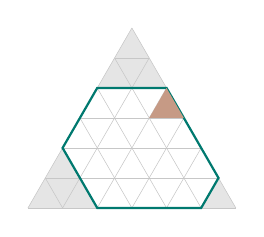
\begin{tikzpicture}[x={(.44cm,0cm)},y={(.22cm,.381cm)}]
\fill[black!10] (0,0)--(2,0)--(0,2)--cycle;
\fill[black!10] (6,0)--(5,0)--(5,1)--cycle;
\fill[black!10] (0,6)--(0,4)--(2,4)--cycle;
\foreach \j in {0,...,6}{
  \draw[black!22,very thin] (\j,0)--(\j,{6-\j});
  \draw[black!22,very thin] (0,\j)--({6-\j},\j);
  \draw[black!22,very thin] (\j,0)--(0,\j);}
\draw[accent,thick] (0,2)--(0,4)--(2,4)--(5,1)--(5,0)--(2,0)--cycle;
\fill[rust!55] (2,3)--(3,3)--(2,4)--cycle;
\end{tikzpicture}
\end{minipage}\hspace{.02\linewidth}
\begin{minipage}{.57\linewidth}\small
For \(a=1,b=2,c=2,d=1\), the outer triangle has side six. The three gray corners are removed. The shaded upward triangle inside the hexagon has index \((2,3,0)\), the single boundary column used below.
\end{minipage}
\end{center}

\clearpage
\subsection*{Proof of Theorem \ref{th:hex}}
Each \(F_l\) has degree \(t\). Its degrees in \(X,Y,Z\) are at most \(b+l+c,\ a+d-1-l+c,\ a+b+d-1\), respectively, which ensure the bounds defining \(V\). It is invariant under simultaneous translation of \(X,Y,Z\), so \((\partial_X+\partial_Y+\partial_Z)F_l=0\). Take the coefficient of a monomial \(X^iY^jZ^k\) of degree \(t-1\) and multiply by \(i!j!k!\). The result says precisely that the corresponding row of \(KH\) vanishes. At \(Z=0\) the form becomes \(Y^{a+d-1-l}X^{b+l}(X-Y)^c\). Thus on the \(d\) boundary vertices \((b+s,t-b-s,0)\), \(0\le s<d\), the restriction \(D\) of \(H\) is lower triangular with diagonal \((-1)^c(b+s)!(t-b-s)!\).

Delete these \(d\) columns of \(K\) to form a square matrix \(A\). We compute its determinant by unit pivots. Set \(C=a+b+d\), so the largest permitted \(k\) is \(C-1\). The unknowns \(h_{i,j,k}\) at undeleted vertices are extended by zero off the region and at deleted vertices. In a row of height \(k<C-1\), eliminate the unique variable directly above it using
\[
 h_{i,j,k+1}=-h_{i+1,j,k}-h_{i,j+1,k}.
\]
Every variable above level zero occurs as such a pivot, with coefficient one, and the other variables in its equation are below it. At the top the rows have \(i+j=c-1\). After substitution their equations, up to row signs, are
\[
 \sum_{p=0}^{C}\binom Cp h_{i+p,t-i-p,0}=0,\qquad 0\le i<c.
\]
Indeed a descent has \(C\) steps which increase either \(i\) or \(j\). If the endpoint is permitted, every intermediate index satisfies both upper bounds by monotonicity. If the endpoint lies outside, its boundary value is zero. The bottom interval before deletion is \(b\le i\le b+d+c-1\). The remaining square matrix is therefore
\[
 \left[\binom{C}{b+d+v-u}\right]_{0\le u,v<c}.
\]
Let \(x=b+d,\ y=a\), so \(C=x+y\). Multiply column \(v\) by \((x+v)!(y+c-1-v)!/C!\). Its entries become evaluations at \(v\) of the polynomials
\[
 f_u(v)=(x+v)_{\underline u}\,(y+c-1-v)_{\underline{c-1-u}},
\]
where the underline denotes a falling factorial. This identity includes zero binomial entries. The polynomials have degree at most \(c-1\). Their evaluation determinant is the determinant of their coefficient matrix times a Vandermonde, hence is invariant under translating all evaluation points by the same amount. Evaluate instead at \(v=-x+j,\ 0\le j<c\). Entries below the diagonal vanish, and entry \(j,j\) is \(j!(C+c-1-j)!/C!\). Dividing out the column multipliers gives \(\Mac(a,b+d,c)\). Lemma \ref{lem:complement} with this minor and the displayed diagonal of \(D\) proves the theorem.\qed

For example \(a=b=c=3,d=1\) gives \(813\,189\,888=2^8\,3^3\,7^6\), as in Propp's paper. For a scalar evaluation in every imbalance, form \(G=H^{\mathsf T}H\), define \(e_0=1\), and iterate the Newton identities
\[
 j e_j=\sum_{k=1}^j(-1)^{k-1} e_{j-k}\tr(G^k),\qquad 1\le j\le d.
\]
Then \(e_d\) is the determinant in Theorem \ref{th:hex}. Every coefficient in \eqref{eq:coeff} is obtained by expanding three binomials. Thus the formula uses only factorials, finite sums and products, and divisions by explicit nonzero integers.

\clearpage
\section{Aztec rectangles of arbitrary width}
Use the points with coordinates of opposite parity in
\([0,2m]\times[0,2n]\), joining diagonal neighbors. Choose \(1\le m\le n\) and put \(d=n-m\). The rows are indexed by \((2i+1,2v)\) and the columns by \((2i,2j+1)\). There are \(m(n+1)\) rows and \((m+1)n\) columns. A quarter turn interchanges the side parameters.

For \(h=\lfloor m/2\rfloor\) and \(k\in\Z\) define the integers
\[
 c_k=(-1)^{|k|}\sum_{j=|k|}^{h}2^{m-2j}\binom{m+1}{2j+1}\binom{2j}{j+k},
 \qquad T_m(t)=\det[c_{i-j}]_{0\le i,j<t}.
\]
\begin{theorem}\label{th:aztec}
The Gram determinant of the \(m\)-by-\(n\) Aztec rectangle is
\[
 \boxed{\displaystyle
 \Gram=2^{m(m+1)}T_m(\lfloor d/2\rfloor)T_m(\lceil d/2\rceil).}
\]
For fixed width \(m\), each \(T_m(t)\) also has the fixed-length finite sum in Theorem \ref{th:roots}.
\end{theorem}
\begin{proof}
Encode column data in \(W_i(z)=\sum_{j=0}^{n-1}w_{ij}z^j\), for \(0\le i\le m\). With \(A=z+\ii,\ B=1+\ii z\), the row polynomials are
\[
 (KW)_i=A W_i+B W_{i+1},\qquad 0\le i<m.
\]
Since \(A,B\) are coprime, the complete kernel is
\begin{equation}\label{eq:layer}
 W_i=(-1)^i A^i B^{m-i}H,\quad \deg H<d.
\end{equation}
Indeed \(B^mW_m=(-A)^mW_0\) gives \(B^m\mid W_0\); write \(W_0=B^mH\) and use the equations successively. Conversely the displayed form solves them. For \(d=0\) only \(H=0\) occurs. Take the columns corresponding to \(H=z^l,\ 0\le l<d\). Their restriction to the first \(d\) coefficients of \(W_0\) is lower triangular with diagonal \(B(0)^m=1\).

Call \(A_0\) the square minor of \(K\) deleting these boundary columns. If \(d>0\), the constant of \(W_0\) is deleted. The \(m\) constant output equations have coefficient one on each new variable \(W_{i+1}(0)\) and depend only on it and \(W_i(0)\). Eliminate these constants with unit pivots. The restricted inputs and outputs are now divisible by \(z\). Dividing by \(z\) leaves exactly the same minor with \(n\) replaced by \(n-1\). Thus \(|\det A_0|\) equals its value for \(n=m\), the balanced Aztec diamond. By the Aztec diamond theorem \cite{eklp}, this value is \(2^{m(m+1)/2}\).

For a direct algebraic derivation of that normalization, homogenize \(A=z+\ii w,\ B=w+\ii z\). The square map sends \(m+1\) binary forms of degree \(m-1\) to \(m\) forms of degree \(m\). In independent variables \(A,B\) its integer matrix has determinant \(\pm1\). Over every prime field the equation \(B^m W_m=(-A)^m W_0\) forces \(W_0=0\) by degree, and then forces all \(W_i=0\). Consequently no prime divides the determinant. On forms of degree \(j\), substitution by the linear change \((z,w)\mapsto(A,B)\) has determinant \(2^{j(j+1)/2}\): triangularize the two-variable substitution and multiply the \(j+1\) diagonal monomial eigenvalues. The ratio of the output and input change-of-basis determinants is \(2^{m(m+1)/2}\), as claimed.

\clearpage
The coefficient inner product of polynomials is the constant Laurent coefficient of their product after conjugating the first on the unit circle. By \eqref{eq:layer}, the Gram matrix of the kernel columns is Toeplitz with symbol
\[
 S_m(z)=\sum_{i=0}^m |z+\ii|^{2i}|1+\ii z|^{2(m-i)}.
\]
For \(z=e^{\ii\theta}\) and \(s=\sin\theta\), the squared moduli are \(2+2s,\ 2-2s\). Summing the geometric progression gives
\[
 S_m(z)=\frac{(2+2s)^{m+1}-(2-2s)^{m+1}}{4s}
   =h_m(z^2),\qquad
 h_m(y)=\sum_{j=0}^h2^{m-2j}\binom{m+1}{2j+1}(2-y-y^{-1})^j .
\]
The first equality at \(s=0\) is understood by continuity. The coefficient of \(y^k\) in \((2-y-y^{-1})^j\) is \((-1)^k\binom{2j}{j+k}\). Odd displacements in the original Toeplitz matrix vanish. Reorder even and odd indices to get the two blocks in the theorem. Lemma \ref{lem:complement} and the preceding minor finish the proof.
\end{proof}

\begin{theorem}[Finite root formula]\label{th:roots}
Put \(\alpha=2^{m-2h}\binom{m+1}{2h+1}\). Let \(\mathcal R\) consist of the \(2h\) numbers
\[
 r_{j,\pm}=(\sec\theta_j\pm\tan\theta_j)^2,\qquad
 \theta_j=\frac{j\pi}{m+1},\qquad 1\le j\le h.
\]
Then, for \(t\ge0\),
\[
 T_m(t)=\alpha^t\sum_{\substack{S\subseteq\mathcal R\\|S|=h}}
 \frac{\prod_{r\in S}r^{t+h}}{\prod_{r\in S,\,u\in\mathcal R\setminus S}(r-u)}.
\]
\end{theorem}
\begin{proof}
The nonzero finite roots of \((1+s)^{m+1}-(1-s)^{m+1}\) satisfy \(s^2=-\tan^2\theta_j\), by taking \((1+s)/(1-s)\) to be a nontrivial \((m+1)\)-st root of unity. The value \(-1\) of that quotient is impossible for finite \(s\). As \(4s^2=2-y-y^{-1}\), the roots in \(y\) are precisely \(\mathcal R\). They are distinct, positive and reciprocal in pairs, because \(0<\theta_j<\pi/2\) and \(\sec\theta+\tan\theta\) is strictly increasing there. Comparing the leading coefficients gives
\[
 y^h h_m(y)=(-1)^h\alpha\prod_{r\in\mathcal R}(y-r),\quad
 c_k=(-1)^k\alpha e_{h-k}(\mathcal R),
\]
where \(e_i\) is the elementary symmetric polynomial, set to zero outside \(0\le i\le2h\). The row and column signs cancel in \(T_m(t)\). The dual Jacobi--Trudi identity \cite[Ch.~I, \S3]{macdonald} gives
\(\det[e_{h-i+j}]_{0\le i,j<t}=s_{(t^h)}(\mathcal R)\).
In the alternant formula for this rectangular Schur polynomial, the top \(h\) exponents are \(t+h,\ldots,t+2h-1\) and the others \(0,\ldots,h-1\). Expand the numerator along the rows of the high exponents. The two internal Vandermonde products cancel those in the denominator, leaving the displayed cross differences and powers. This also gives \(1\) when \(h=0\) after removing \(\alpha^t\).
\end{proof}
The largest exponential base is unique, from all \(h\) roots greater than one; its coefficient is positive. Hence \(\lim_{n\to\infty}\Gram^{1/n}=\alpha\prod_{j=1}^h r_{j,+}\) for fixed \(m\). Width one gives \(\Gram=4^n\). For \(m=4\) the values at \(n=5,9\) are \(174\,063\,616\) and \(105\,718\,590\,996\,480\,000\).

\clearpage
\section{The eigenvalue four on an Aztec rectangle}
Saldanha exhibited a factor \((t-4)^{4k}\) in examples of order \(2k+1\) and asked for its explanation \cite[\S6]{saldanha}. The boundary equations yield the multiplicity on the full rectangular family.
\begin{theorem}\label{th:four}
On the \(m\)-by-\(n\) Aztec rectangle, \(1\le m\le n\), the multiplicity of \(4\) in \(KK^*\) is
\[
 (m\bmod2)(n-1)+(n\bmod2)(m-1).
\]
In particular it is \(4k\) for an Aztec diamond of order \(2k+1\), and zero for every even order.
\end{theorem}
\begin{proof}
Let \(U\) be the \(m\)-by-\(m\) upper shift, \(P=U+U^*\), \(J=U-U^*\), and \(B_\pm=2I\pm\ii J\). These last two matrices are positive definite. Conjugating \(\ii J\) by a diagonal matrix of powers of \(\ii\) yields a signed path adjacency with all eigenvalues strictly between \(-2\) and \(2\). Moreover \(\delta=\dim\ker P=m\bmod2\), by the path eigenvalues in Theorem \ref{th:fool}.

Write a row-space vector by its \(n+1\) coefficient levels \(x_0,\ldots,x_n\in\C^m\). The equation \(KK^*x=4x\) is
\begin{equation}\label{eq:four}
 P(x_{j-1}+x_{j+1})=0\ (1\le j<n),\qquad
 Px_1=B_+x_0,\quad Px_{n-1}=B_-x_n .
\end{equation}
To verify it, the diagonal block from the two incidence polynomials \(A,B\) is \(AA^*+BB^*\), with diagonal entries \(2,4,\ldots,4,2\) and zero off-diagonal entries. The upper block between consecutive row chains is \(BA^*\). Its neighboring diagonals are \(1\), and its main diagonal is \(-\ii,0,\ldots,0,\ii\). The lower block is its adjoint. Collecting these entries gives \eqref{eq:four}, including \(n=1\).

Set \(y_j=Px_j\). In the interior \(y_{j+1}=-y_{j-1}\). For any admissible endpoints \(x_0,x_n\) the endpoint equations determine all the \(y_j\), including \(y_1\). Each interior \(x_j\) can then be lifted independently, with \(\delta\) free coordinates. It remains to count admissible endpoints.

If \(n\) is odd, put \(\sigma=(-1)^{(n-1)/2}\). Then \(y_1=\sigma y_n,\ y_{n-1}=\sigma y_0\), and the endpoint pairs are precisely the kernel of
\[
 \begin{pmatrix}B_+&-\sigma P\\-\sigma P&B_-\end{pmatrix}.
\]
Here all the \(y_j\) are automatically in the image of \(P\). Grouping the two endpoint coordinates at each path site rewrites the displayed matrix as \(2I+U\otimes M+U^*\otimes M^*\), with
\[
 M=\begin{pmatrix}\ii&-\sigma\\-\sigma&-\ii\end{pmatrix}
   =2ef^*,\quad e=(\ii,-\sigma)^{\mathsf T}/\sqrt2,\quad
 f=(1,-\ii\sigma)^{\mathsf T}/\sqrt2.
\]
The vectors \(e,f\) are orthonormal. In this basis the operator has \(m-1\) disjoint blocks
\(\left(\begin{smallmatrix}2&2\\2&2\end{smallmatrix}\right)\) on \(e_j,f_{j+1}\) and two singleton entries \(2\). The endpoint nullity is \(m-1\).

If \(n\) is even, let \(\eta=(-1)^{n/2}\) and set \(w=\eta x_n\). The recurrence and endpoints give \(P(w-x_0)=0,\ B_-w=-B_+x_0\). As \(B_+x_0=Px_1\) is perpendicular to \(\ker P\), one has
\(\langle x_0,B_+x_0\rangle=\langle w,B_+x_0\rangle=-\langle w,B_-w\rangle\).
Positivity forces \(w=x_0=0\). This leaves only the \((n-1)\delta\) interior coordinates. In both parity cases the count is the algebraic multiplicity because \(KK^*\) is Hermitian.
\end{proof}

\clearpage
\section{Historical values and verification}
The first eight values of \(R_{n-1,n-1}\) reproduce Propp's entire list \cite[p.~283]{propp}. The last two below extend that table using \eqref{eq:resultant}. The cosine products were already proposed by Manyama, and the odd-index values also occur in A340291 \cite{oeis}.
\begin{center}
\begin{tabular}{@{}r r @{\qquad\qquad}r r@{}}
\toprule \(n\)&\(R_{n-1,n-1}\)&\(n\)&\(R_{n-1,n-1}\)\\\midrule
1&1&6&9\,085\,440\\
2&2&7&8\,238\,791\,743\\
3&15&8&24\,233\,379\,889\,152\\
4&384&9&230\,629\,380\,093\,001\,665\\
5&32\,625&10&7\,089\,727\,956\,532\,936\,704\,000\\\bottomrule
\end{tabular}
\end{center}
Knuth's Theorem 2 gives a second interpretation of the square root \cite{knuth}. Write \(E_{p,q}\) and \(O_{p,q}\) for the two checkerboard parity classes on a \(p\)-by-\(q\) grid with diagonal moves. The adjacency of their union at size \(r,s\) is \(P_r\otimes P_s\). Its spectrum is invariant under sign reversal. Knuth identifies the two characteristic polynomials at \(4\) with the spanning-tree counts of the opposite parity graphs at size \(r+2,s+2\). It follows that
\[
 \Gram(F_{r,s})=\tau(E_{r+2,s+2})\,\tau(O_{r+2,s+2}).
\]
For positive \(r,s\), the tree counts are equal when either enlarged dimension is even (reflect the grid), and have ratio four when both are odd \cite[Cor.~2]{knuth}. This gives another proof that the integer \(\Gram\) is a square. In the honeycomb setting, the monomial description of triangular regions and their biadjacency maps also occurs in work of Cook and Nagel \cite{cook}.

The companion Lean project verifies the determinant identity of Lemma \ref{lem:complement}, the complete matrix-to-product theorem for \(F_{r,s}\), both of Manyama's parity products, the capped three-neighbor equation in the hexagon, and the Aztec polynomial kernel, its unit boundary minor and its symbol identity. Lean also verifies the endpoint change of basis and the dimension of the paired constraints in Theorem \ref{th:four}. The elimination, Toeplitz evaluation and rectangle multiplicity arguments are given in this manuscript. The companion Python program constructs honeycomb adjacency geometrically by shared triangle sides and uses a real square-grid signing. It compares \(373\) independently constructed Gram determinants by exact arithmetic and checks \(63\) exact ranks at eigenvalue \(4\). It separately compares \(80\) root sums and \(15\) parity products at high precision.

{\small
\begin{thebibliography}{9}\setlength{\itemsep}{1pt}
\bibitem{propp} J. Propp, \emph{Enumeration of matchings: problems and progress}, MSRI Publications 38 (1999), 255--291. \href{https://library.slmath.org/books/Book38/files/propp.pdf}{Published chapter}.
\bibitem{knuth} D. E. Knuth, \emph{Aztec diamonds, checkerboard graphs, and spanning trees}, J. Algebraic Combin. 6 (1997), 253--257. \href{https://arxiv.org/abs/math/9501234}{arXiv:math/9501234}.
\bibitem{saldanha} N. C. Saldanha, \emph{Singular polynomials of generalized Kasteleyn matrices}, J. Algebraic Combin. 16 (2002), 195--207. \href{https://arxiv.org/abs/math/0101002}{Preprint, December 2000}.
\bibitem{oeis} OEIS Foundation, \href{https://oeis.org/A071102}{A071102}, including S. Manyama's conjectures of January 4, 2021. Related entries \href{https://oeis.org/A340166}{A340166} and \href{https://oeis.org/A340291}{A340291}.
\bibitem{eklp} N. Elkies, G. Kuperberg, M. Larsen and J. Propp, \emph{Alternating-sign matrices and domino tilings}, J. Algebraic Combin. 1 (1992), 111--132, 219--234. \href{https://arxiv.org/abs/math/9201305}{Preprint}.
\bibitem{macdonald} I. G. Macdonald, \emph{Symmetric Functions and Hall Polynomials}, 2nd ed., Oxford University Press, 1995.
\bibitem{cook} D. Cook II and U. Nagel, \emph{Signed lozenge tilings}, Electron. J. Combin. 24 (2017), P1.9. \href{https://arxiv.org/abs/1507.02507}{arXiv:1507.02507}.
\end{thebibliography}}
\end{document}
